\section{Design}

This section provides an overview of the design aspects of our tool during the third sprint. It includes diagrams that illustrate the system's structure and behavior.

\subsection{Class Diagram}

The class diagram (Figure \ref{fig:Sprint 3 Class Diagram}) visualizes the system's structure. It shows the classes, their attributes and operations, and the relationships among them.

\begin{figure}[ht]
	\centering
	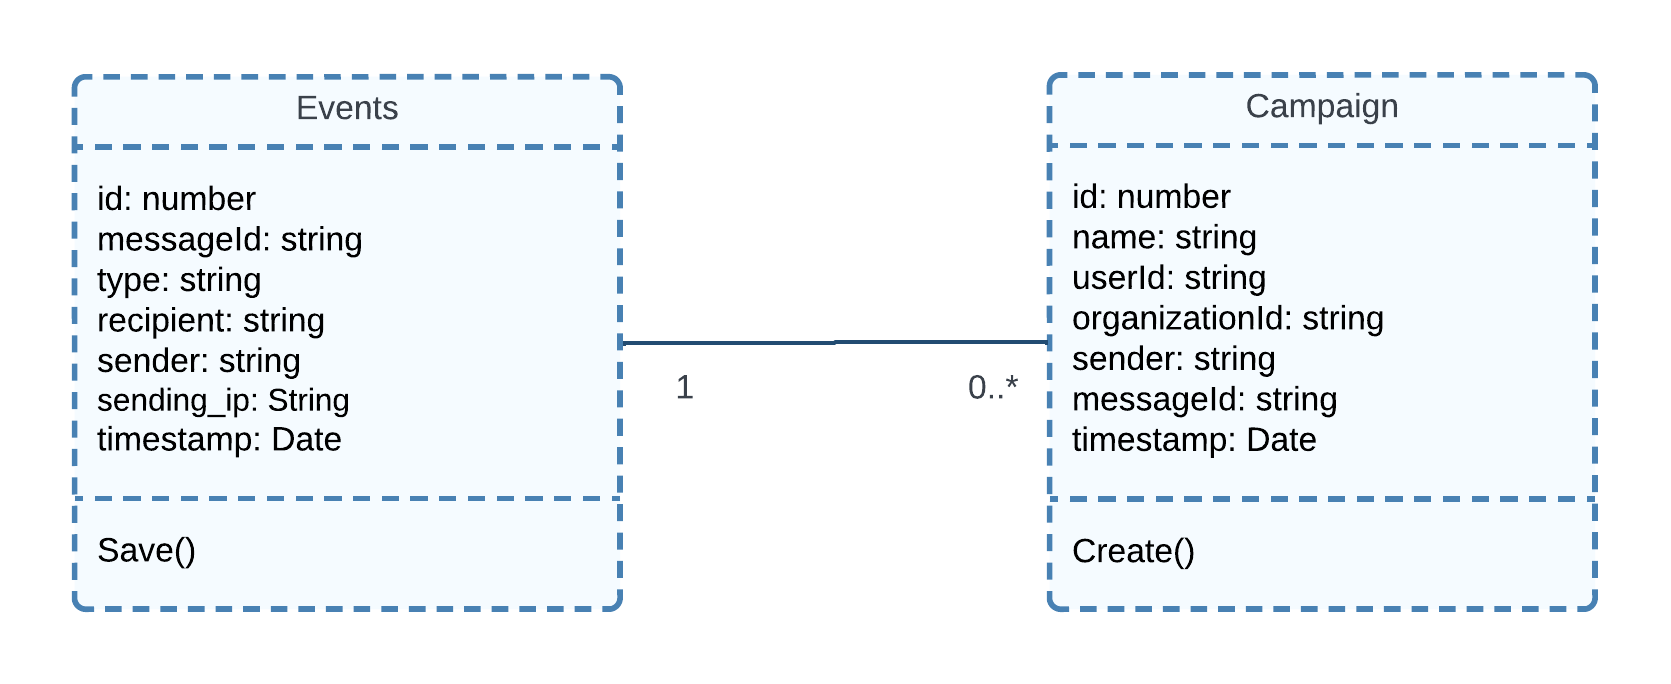
\includegraphics[width=\linewidth]{Images/Sprint3/class diag.png}
	\caption{Sprint 3 Class Diagram}
	\label{fig:Sprint 3 Class Diagram}
\end{figure}

\subsection{Sequence Diagrams}

The sequence diagrams illustrate the flow of operations in the system, emphasizing the interaction between objects over time. Each diagram corresponds to a specific use case or functionality.

\paragraph{Saving Taracking Data Sequence Diagram}

Figure \ref{fig:Sprint 3 Saving Taracking Data Sequence Diagram} describes the scenario of how the Tracking Data is being saved.

\begin{figure}[ht]
	\centering
	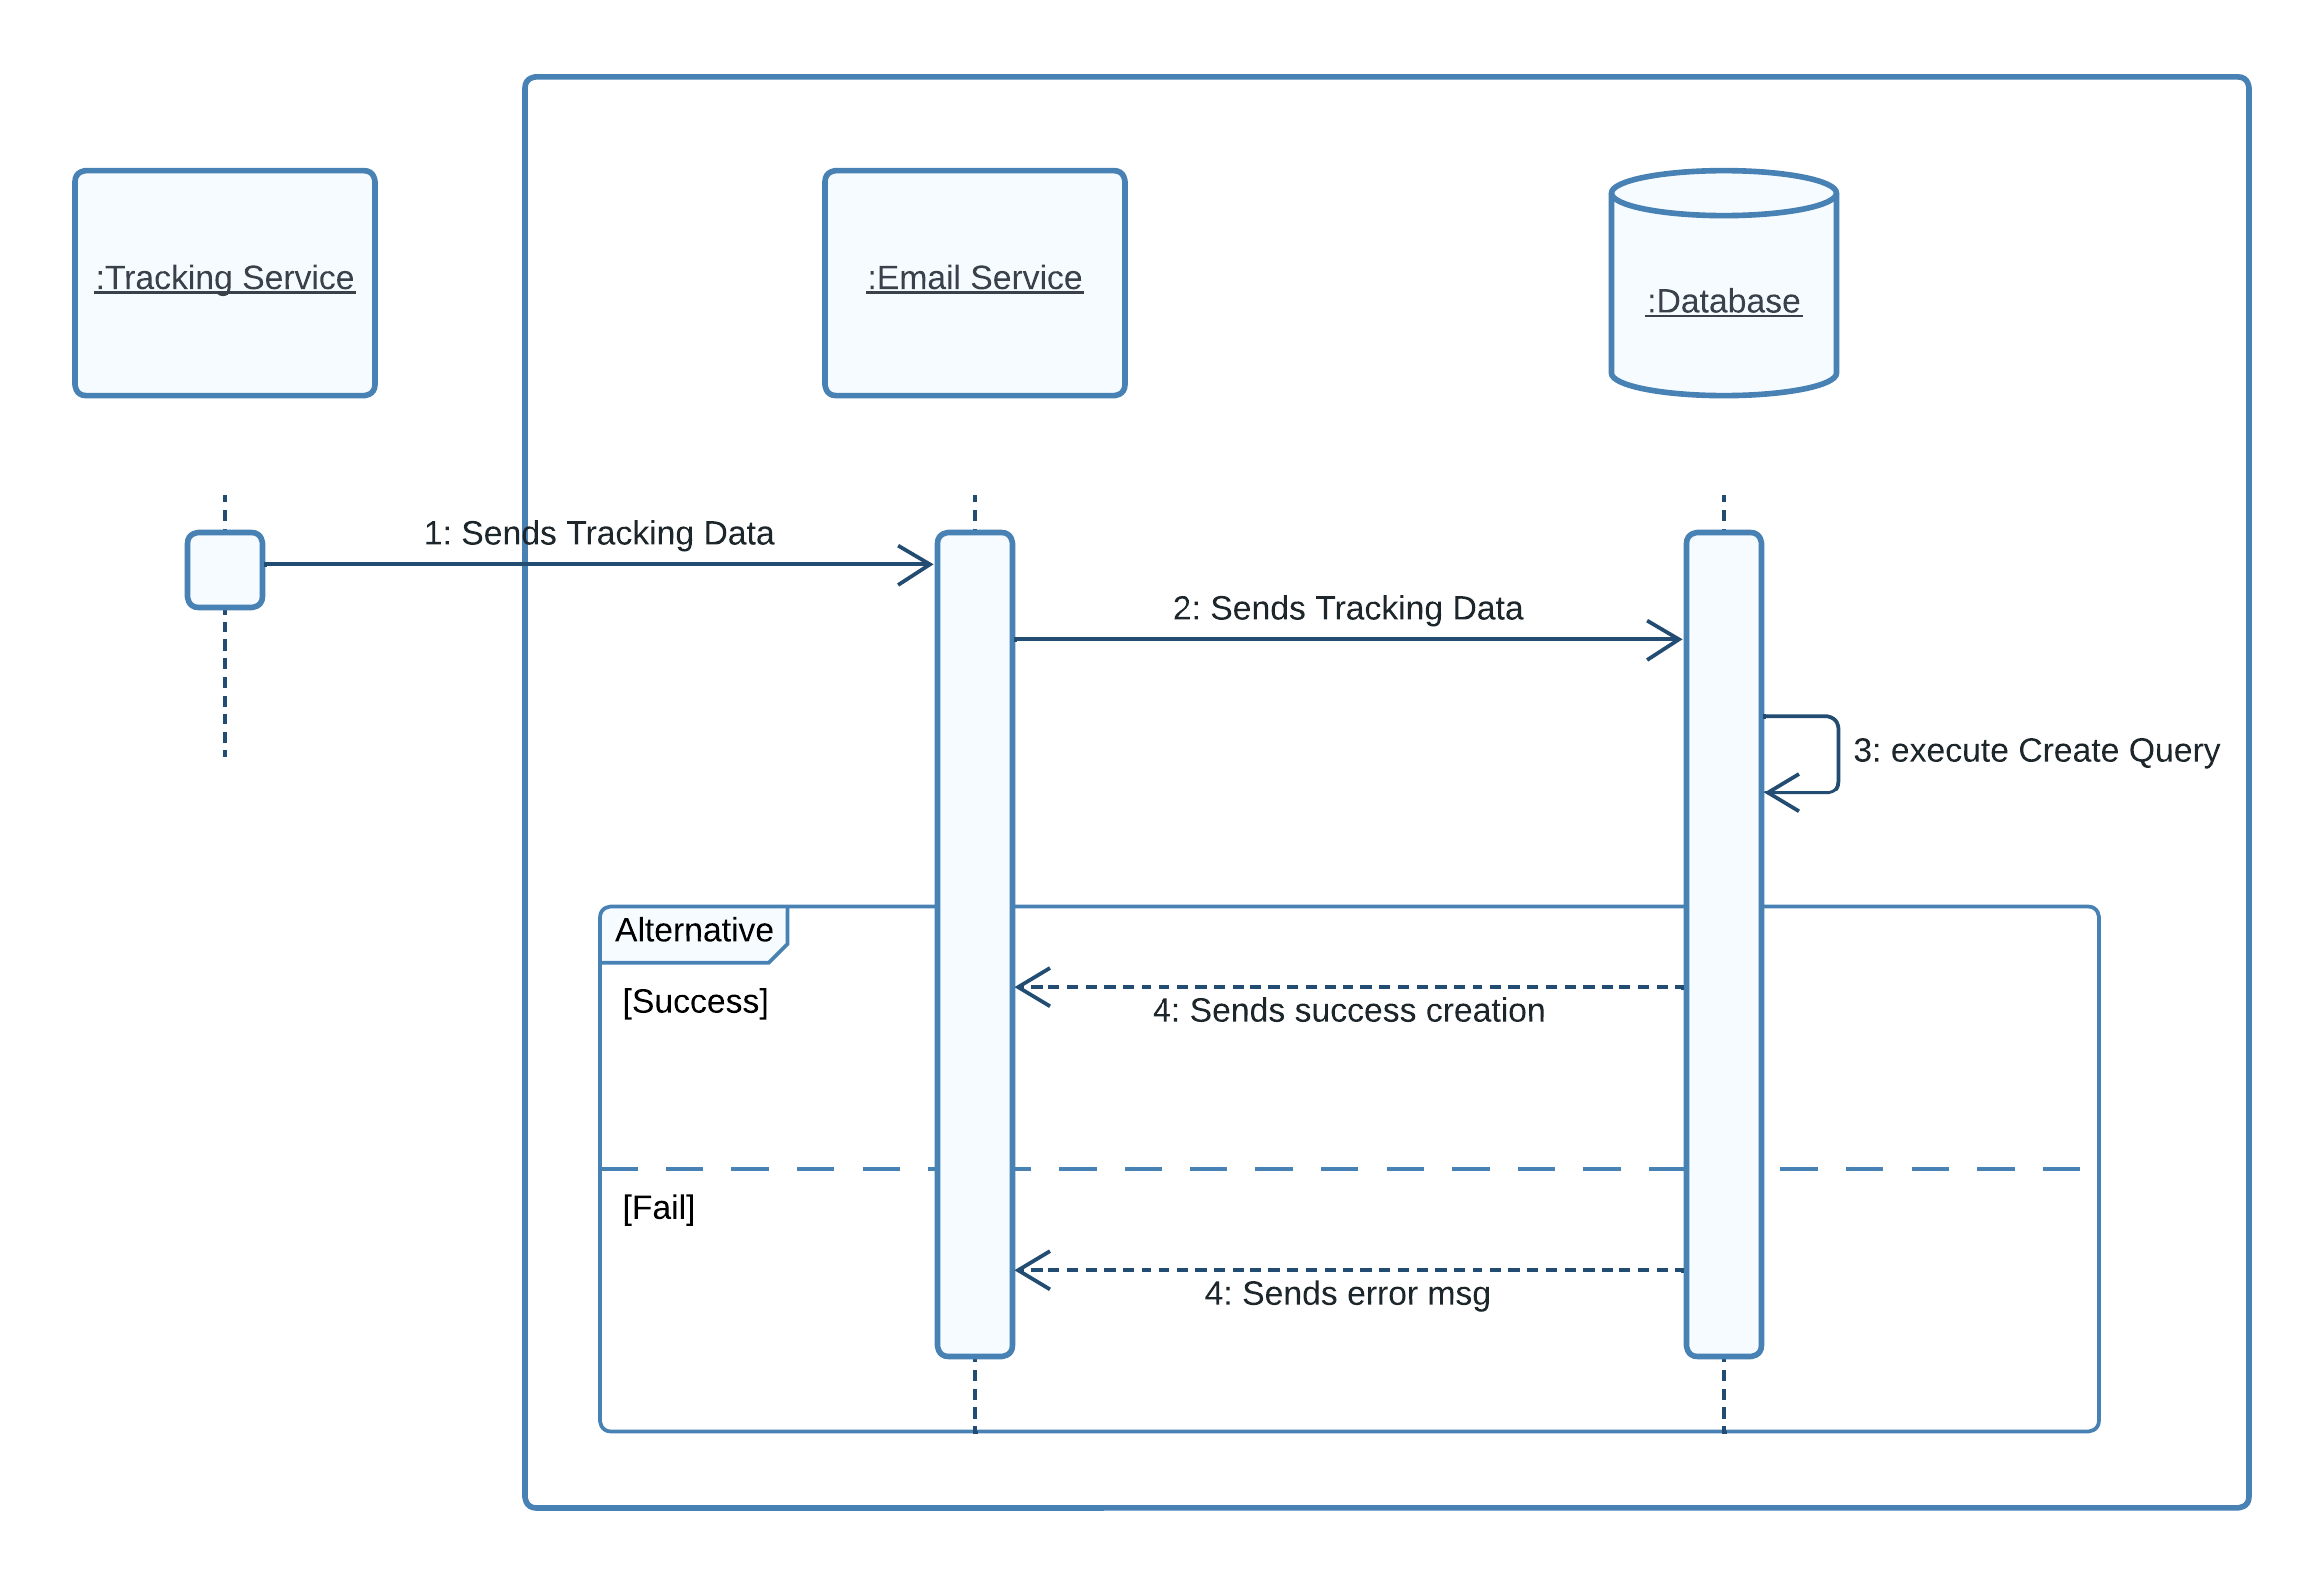
\includegraphics[width=0.8\linewidth]{Images/Sprint3/sequence diag sprint 3/tracking insights sequence diag.png}
	\caption{ Tracking Sequence Diagram}
	\label{fig:Sprint 3 Saving Taracking Data Sequence Diagram}
\end{figure}

\paragraph{ Taracking Insights Sequence Diagram}

Figure \ref{fig:Sprint 3 Taracking Insights Sequence Diagram} describes the scenario of how the Tracking Insights is being handeled.

\begin{figure}[ht]
	\centering
	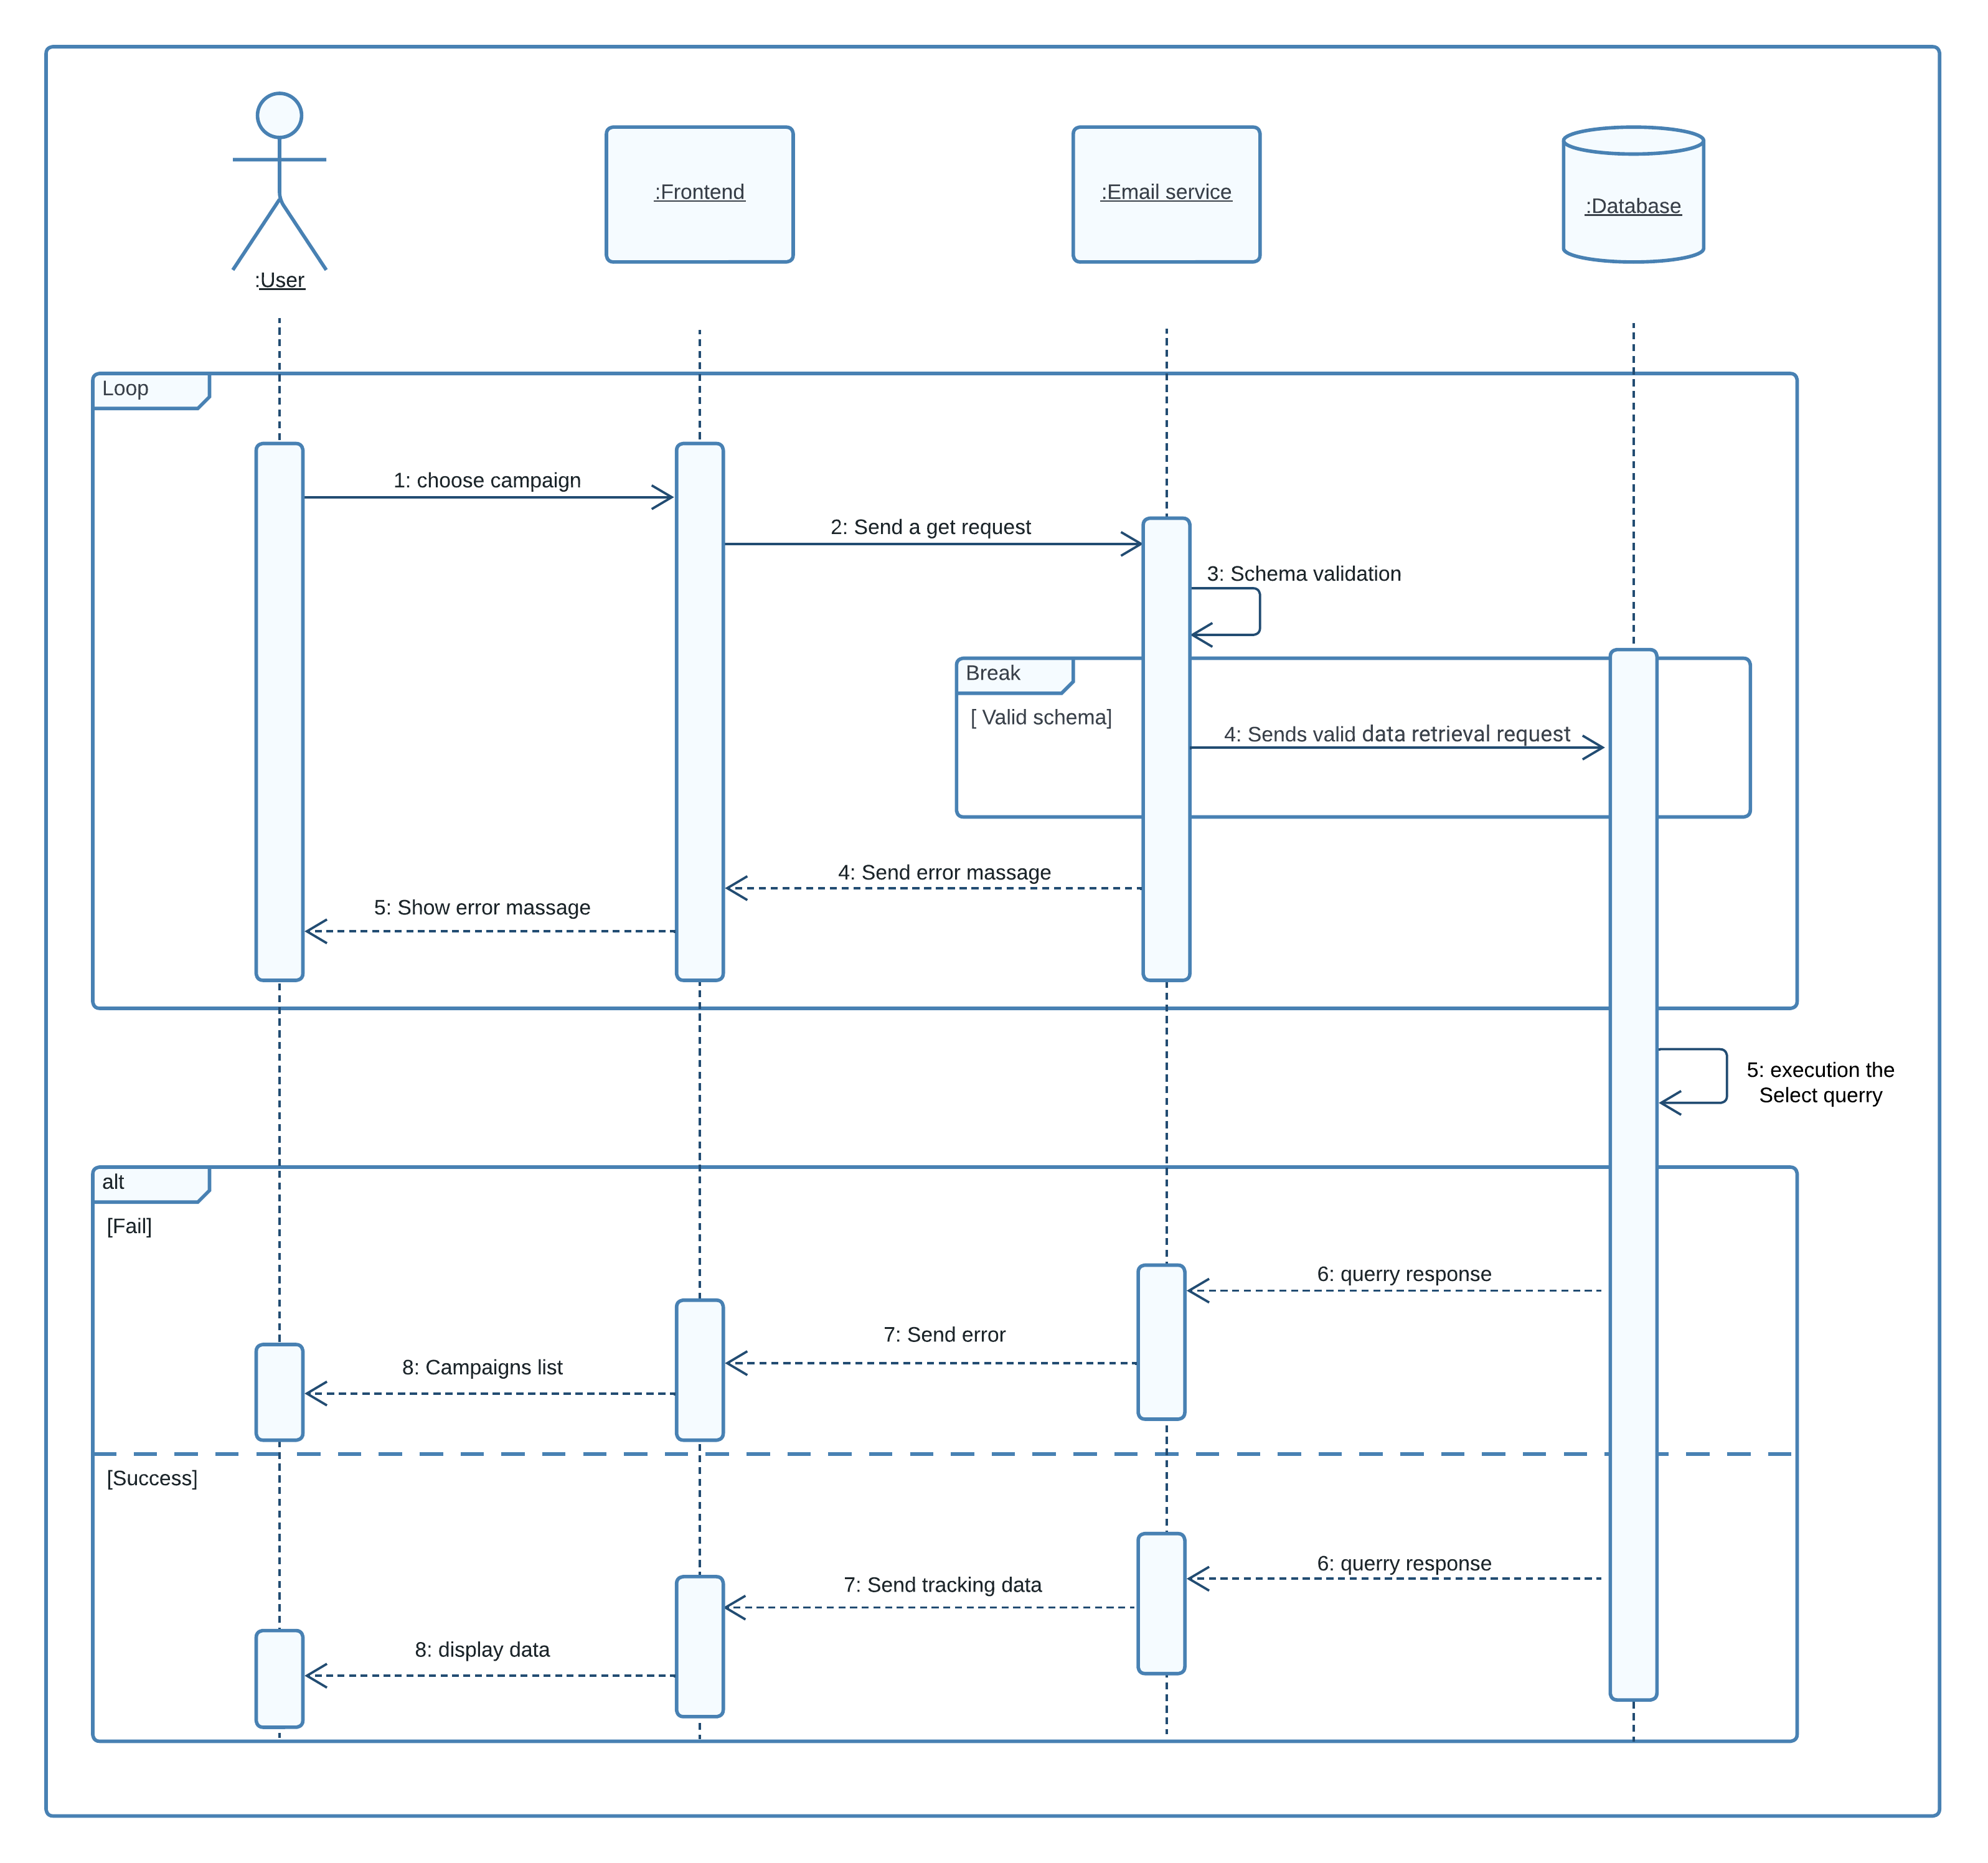
\includegraphics[width=\linewidth]{Images/Sprint3/sequence diag sprint 3/view insights.png}
	\caption{ Tracking Sequence Diagram}
	\label{fig:Sprint 3 Taracking Insights Sequence Diagram}
\end{figure}

\clearpage